%% IPM --- Elsevier elsarticle (authors in frontmatter under the title; titlepage mirrors the same block)
\documentclass[preprint,12pt,authoryear]{elsarticle}

\usepackage{amssymb,amsmath}
\usepackage{graphicx}
\usepackage{booktabs}
\usepackage{multirow}
\usepackage{array}
\usepackage{xurl}
\usepackage{microtype}
\usepackage{placeins}
\usepackage{float}
\usepackage{lineno}
\usepackage{algorithm}
\usepackage{algpseudocode}
\usepackage{amsthm}
\usepackage[hidelinks]{hyperref}
\newtheorem{definition}{Definition}
\newtheorem{proposition}{Proposition}
\newtheorem{remark}{Remark}
\graphicspath{{figures/}}
\DeclareUrlCommand\codeid{\urlstyle{tt}}
\newcommand{\tbd}{---}
% Compact tables: never stretch with \resizebox (avoids oversized, eye-catching grids).
\newcommand{\compacttab}{\setlength{\tabcolsep}{4.5pt}\renewcommand{\arraystretch}{1.05}}

\journal{Information Processing \& Management}

\begin{document}

\begin{frontmatter}

\title{BIMS-LEGAL: Dual-Store Soft Binding for Recovering Prior Legal Advice under Same-Domain Interference}

%% Author names and affiliations appear under the title (IPM/Elsevier frontmatter),
%% not at the end of the article. End-matter CRediT is a contribution statement only.
\author[]{Anonymous Author(s)}
\ead{anonymous@anonymous.edu}

\begin{abstract}
\sloppy
Recovering prior client-specific advice from a legal consultation archive is difficult because dense retrieval may rank a relevant question turn highly while omitting the lawyer's answer---an \emph{episode incompleteness} failure under same-domain interference.
BIMS-LEGAL is a dual-store system for Chinese legal consultation logs: a fast episodic turn index with session identifiers and a slower BIRCH semantic store.
Soft~O2 performs turn-level session binding by giving siblings attenuated inherited scores ($\beta s$) rather than hard score copy.
We evaluate exact replay as diagnostic and use paraphrase, follow-up, and advice-recall as primary non-exact channels.
BM25-joint is a strong lexical baseline on exact and high-overlap queries, but Soft~O2 is more effective on non-exact channels where online turn-level retrieval can recover a partial episode and then bind its answer sibling.
Soft~O2-C and gated Hybrid are reported as exploratory, gold-assisted solvability bounds for cross-session recovery, not as claims about natural unsupervised deployment.
We report corrected graded nDCG alongside Answer Hit and Episode Completeness, with paired significance tests and a failure taxonomy separating complete, incomplete, and missed-session retrieval.
\end{abstract}

\begin{keyword}
legal information retrieval \sep consultation memory \sep soft episode binding \sep dual-store memory \sep cluster binding \sep Chinese legal corpora
\end{keyword}

\end{frontmatter}

\linenumbers

\section{Introduction}\label{sec:intro}

A junior associate may ask a firm assistant: ``Last month you advised this client on terminating a fixed-term contract---what remedy did we recommend?'' The system returns several near-identical ``contract termination'' questions, ranks the stored user utterance highly, and never surfaces the partner's written advice. The subsequent reply may sound fluent yet be grounded in the wrong episode---or in none. In consultation archives, questions and answers share specialized terminology; neighbouring matters are topically adjacent yet legally distinct; and the professionally useful evidence unit is the full consultation \emph{episode}.

Legal informatics has long studied statutory interpretation, case retrieval, and advisory systems \cite{martinezgil2023survey, ashley2017artificial}.
Recent legal large language models (LLMs) improve statutory and fact-pattern answering \cite{yue2023disclawllm, huang2023lawyer, yue2024lawllm}.
Classical legal information retrieval (IR) mainly targets \emph{external} authority---statutes, cases, or community answers---as documents \cite{askari2024legalqa, louis2024lleqa, liu2022query, zhang2024event}.
Memory-augmented dialogue systems recover evidence from evolving conversation logs \cite{wu2025longmemeval, maharana2024evaluating, packer2023memgpt}.
The gap addressed here is \emph{internal consultation memory}: retrieving prior client-specific advice from a growing same-domain archive under lexical interference.

BIMS-LEGAL is a dual-store Brain-Inspired Memory System for legal consultation archives, designed and evaluated in this study.
The \emph{systemic contribution} is a dual-store architecture that separates a fast episodic pathway (timestamped turn embeddings with speaker role and session identifier $sid$) from a slow semantic pathway based on Balanced Iterative Reducing and Clustering using Hierarchies (BIRCH) with deferred consolidation \cite{zhang1996birch}.
Complementary Learning Systems (CLS) theory \cite{mcclelland1995complementary, kumaran2016} supplies an architectural analogy for this dual-pathway design, not an empirical claim about biological memory.
Under same-domain interference, dense turn retrieval in a vector database often returns a question turn while its answer sibling remains outside top-$k$---a system-level episodic memory failure we term \emph{episode incompleteness}, distinct from a full session miss and exacerbated by IVFPQ score collapse and context fragmentation at moderate archive sizes.

The \emph{algorithmic contributions} are soft binding operators that complete episodes without hard score copy:
\begin{itemize}
    \item \textbf{Soft~O2 (session soft binding).} When a turn is retrieved with score $s$, siblings sharing $sid$ inherit $\max(s_{t'},\,\beta\cdot s)$, surfacing answer turns under question-hit~/~answer-miss while preserving rank competition among candidates.
    \item \textbf{Soft~O2-C and gated Hybrid (cluster soft binding).} The same soft-inheritance rule applies within BIRCH clusters when gold evidence is not co-session with the query; Hybrid triggers cluster binding only on direct dense hits to avoid displacing same-session siblings.
\end{itemize}
Two \textbf{implementation and scale design operators} support rigorous large-scale shared-store experiments but are not standalone algorithmic contributions:
\begin{itemize}
    \item \textbf{O1 (exact FlatIP indexing).} At hundreds-to-thousands of turns, IVFPQ product quantization is under-trained and collapses Answer Hit; FlatIP restores faithful turn scores so Soft~O2 inherits uncorrupted sibling signals.
    \item \textbf{O3 (bulk-load consolidation).} Deferred BIRCH and disk writes make archive construction tractable without changing retrieval semantics.
\end{itemize}

We ask four research questions:

\begin{itemize}
    \item \textbf{RQ1.} Under same-domain interference, does episode incompleteness (question hit~/~answer miss) dominate full session miss?
    \item \textbf{RQ2.} Do Soft~O2 and Soft~O2-C address episode incompleteness under measured index distortion, and what incremental gains does Soft~O2 provide over FlatIP and hard parent hydration?
    \item \textbf{RQ3.} On the \emph{same} LegalEp~/LegalMem stores, when is the slow (BIRCH) pathway effective? Does Soft~O2-C help under standard same-session gold, and under a fair Mix of same-/cross-session gold?
    \item \textbf{RQ4.} Across CAIL multi-turn and LegalEp paraphrase~/advice-recall channels, how large and session-tied are Soft~O2 gains, and how do Soft~O2 and Soft~O2-C~/Hybrid complement each other?
\end{itemize}

\paragraph{Contributions.}
\begin{enumerate}
    \item A dual-store memory architecture for Chinese legal consultation archives, separating fast episodic turn recovery from slower BIRCH semantic integration under same-domain interference.
    \item Soft~O2, a turn-level session soft-binding operator that addresses episode incompleteness without hard parent hydration or session-max score copy.
    \item A conservative three-candidate diagnostic of Soft~O2 score competition using the gap ratio $\rho=s_d/s_h$; default $\beta{=}0.98$ is chosen by validation sweep, not by a closed-form optimum.
    \item An honest comparison with strong lexical baselines: BM25-joint and dense joint-episode indexing are highly competitive on exact/surface-overlap channels, while Soft~O2 targets paraphrase, follow-up, and advice-recall under an online turn-level index.
    \item Exploratory Soft~O2-C / gated Hybrid results under a gold-assisted Mix solvability bound, plus corrected nDCG, failure taxonomy, and paired significance reporting.
    \item O1 exact FlatIP and O3 bulk-load consolidation as implementation operators enabling the shared-store ablations reported here.
\end{enumerate}

Section~\ref{sec:related} reviews related work.
Section~\ref{sec:method} presents BIMS-LEGAL operators and the Soft~O2 diagnostic model.
Section~\ref{sec:protocol} details corpora, corrected metrics, and protocols.
Section~\ref{sec:experiments} reports results.
Section~\ref{sec:discussion} discusses implications and limitations.
Section~\ref{sec:conclusion} concludes.

\section{Related Work}\label{sec:related}

\subsection{Legal IR and long-horizon dialogue memory}
Legal QA and retrieval systems typically ground generation in statutes, cases, or published advice \cite{louis2024lleqa, askari2024legalqa, martinezgil2023survey, ashley2017artificial}.
Conversational legal case retrieval and event-aware similar-case ranking further show how interaction context and structured legal knowledge shape IR effectiveness \cite{liu2022query, zhang2024event}.
Those pipelines optimize access to external authority.
Consultation memory retrieval targets a different evidence source: \emph{prior consultation episodes} inside an agent's own archive.
Confusing two clients' histories can produce fluent yet professionally inappropriate responses even when statute retrieval is correct.
Domain LLMs such as DISC-LawLLM, Lawyer~LLaMA, and LawLLM improve statutory and advisory generation \cite{yue2023disclawllm, huang2023lawyer, yue2024lawllm}, but they still need a reliable memory index when prior advice must be recovered from a growing same-domain log.

Legal consultation archives add a further difficulty: high lexical overlap among topically adjacent matters, with the professionally useful evidence unit being the full question--answer episode.
This setting motivates \emph{dual-store} memory architectures that keep fast episodic turn retrieval separate from slower semantic clustering, and session-aware soft binding operators that recover answer turns under same-domain interference without collapsing rank competition among unrelated candidates.

\subsection{Dual-store memory and episodic retrieval}
Dual-store designs distinguish fast episodic encoding from slower semantic integration \cite{mcclelland1995complementary, kumaran2016, tulving1972episodic, atkinson1971control}.
Memory architectures for dialogue agents extend context via hierarchical paging, summary banks, graphs, and neuro-symbolic retrieval \cite{packer2023memgpt, zhong2024memorybank, rasmussen2025zep, gutierrez2024hipporag, modarressi2023ret, wang2024memoryllm, lewis2020rag, wu2025memory}, but most treat retrieved units as flat passages rather than \emph{multi-turn consultation episodes} whose answer turn may rank below an unrelated question turn sharing legal vocabulary.
LongMemEval and LoCoMo evaluate long-horizon recall and QA over personal conversation logs \cite{wu2025longmemeval, maharana2024evaluating}, while broader memory-agent surveys emphasize persistence beyond the context window \cite{wu2025memory, Tan2025}.
Recent conversational RAG work stresses reuse of historical search evidence across turns \cite{mo2026historical}.
BIMS-LEGAL positions its dual-store contribution at this intersection: episodic turn embeddings with $sid$ for same-session recovery (Soft~O2), and BIRCH centroids with Soft~O2-C for cross-session recovery when query and gold evidence occupy different sessions but share thematic structure \cite{zhang1996birch}.
Soft~O2 directly addresses the episodic retrieval challenge that parent-document hydration and session-max aggregation handle via hard score copy: under dense same-domain interference, a question turn can dominate top-$k$ while its answer sibling remains absent, producing fluent yet ungrounded downstream generation unless siblings enter under attenuated inherited scores.

\subsection{Session-aware retrieval}
Parent-document hydration, session aggregation, and joint session indexing are standard session-aware mechanisms for attaching sibling context to a dense hit.
Soft episode binding (Soft~O2) inherits $\beta\cdot s$ for siblings and keeps ranking competition among candidates. Parent-document and hierarchical retrieval similarly attach child evidence to a parent unit \cite{callan1994passage,dai2019context,zaheer2017deep,karpukhin2020dpr}; Soft~O2 differs by using attenuated turn-level score propagation rather than hard hydration or atomic session documents.
Lexical BM25 \cite{robertson2009bm25}, dense passage retrieval \cite{karpukhin2020dpr}, dense--sparse Reciprocal Rank Fusion \cite{cormack2009rrf}, and cross-encoder reranking \cite{nogueira2019multistage, chen2024bge} provide complementary controls outside session membership.
Exact flat indexes and product-quantized ANN backends \cite{johnson2019billion} further affect whether sibling binding is applied over faithful turn scores.
Table~\ref{tab:rw_compare} summarizes the session-structure contrasts used in the main grids.

\begin{table}[htbp]
\centering
\caption{Session-aware mechanisms compared in this work.}
\label{tab:rw_compare}
\compacttab\footnotesize
\begin{tabular}{@{}llp{2.2cm}cc@{}}
\toprule
\textbf{Mechanism} & \textbf{Unit} & \textbf{Expansion} & \textbf{Type} & \textbf{Rank} \\
\midrule
Parent hydration & Session & Insert siblings & Hard & No \\
Session-max & Session & Session $\max$ & Hard & Same$^*$ \\
Joint episode index & Session doc & Atomic & N/A & N/A \\
Soft O2 & Turn+$sid$ & Soft $\beta s$ & Soft & Yes \\
Soft O2-C & Turn+cluster & Soft $\beta_c s$ & Soft & Yes \\
\bottomrule
\end{tabular}
\end{table}
{\footnotesize $^*$On the reported corpora, session-max rankings coincide with hard parent hydration under full-sibling expansion; main tables report a single hard-expansion baseline. Soft~O2 denotes session soft binding; Soft~O2-C denotes cluster soft binding on the BIRCH pathway.}

We reuse CLS vocabulary as an architectural analogy for BIMS-LEGAL: turn embeddings with timestamps, roles, and session identifiers as episodic elements; Soft~O2 as episode binding on the episodic pathway; BIRCH centroids with Soft~O2-C as semantic integration on the slow pathway; and shared-store distractors as interference.
The dual-store split is the systemic design; Soft~O2 and Soft~O2-C are the algorithmic mechanisms evaluated on Chinese legal consultation archives.

\section{Method: BIMS-LEGAL}\label{sec:method}

\subsection{Architecture overview}
Figure~\ref{fig:bims_architecture} summarizes the pipeline.
BIMS-LEGAL maintains complementary episodic and semantic stores over the same consultation archive.

\begin{definition}[Episodic and semantic elements]\label{def:elements}
An episodic element is $e_i=(\mathbf{v}_i,t_i,c_i,\phi_i,sid_i)$, where $\mathbf{v}_i\in\mathbb{R}^d$ is an embedding, $t_i$ a timestamp, $c_i$ conversational context (including speaker role), $\phi_i$ surface features, and $sid_i$ the consultation session identifier.
A semantic element is $s_j=(\mathbf{c}_j,C_j,\kappa_j,\tau_j)$ with centroid $\mathbf{c}_j$, member set $C_j$, label $\kappa_j$, and formation statistics $\tau_j$.
Write $\mathrm{Sib}(t)=\{t':sid_{t'}=sid_t\}\setminus\{t\}$ for session siblings and $\mathrm{Clus}(t)=\{t':cid_{t'}=cid_t\}\setminus\{t\}$ for BIRCH-cluster siblings.
\end{definition}

\begin{definition}[Dual-store retrieval map]\label{def:retrieval}
Given query $q$ with embedding $\mathbf{v}_q$, base episodic retrieval returns a scored candidate set $\mathcal{R}_0(q)=\{(t,s_t)\}$ under Eq.~\eqref{eq:base-score}.
Soft~O2 produces $\mathcal{R}_{\mathrm{O2}}(q)=\mathsf{SoftBind}(\mathcal{R}_0(q);\mathrm{Sib},\beta)$ (Section~\ref{sec:soft-o2}).
Soft~O2-C produces $\mathcal{R}_{\mathrm{O2C}}(q)=\mathsf{SoftBind}(\mathcal{R}_0(q);\mathrm{Clus},\beta_c)$ (Section~\ref{sec:soft-o2c}).
Gated Hybrid composes session binding then cross-session cluster binding (Algorithm~\ref{alg:hybrid}).
The returned list is the top-$k$ of the bound set under the rewritten scores.
\end{definition}

\begin{figure}[t]
    \centering

\includegraphics[width=0.98\linewidth]{fig1_architecture.png}
\caption{BIMS-LEGAL dual-store pipeline. (A)~Episodic turn indexing and BIRCH semantic clustering (O3 bulk-load consolidation). (B)~Query-time dense retrieval under O1 FlatIP with Soft~O2 session binding and Soft~O2-C cluster binding (algorithmic core); O1 and O3 are implementation operators. (C)~Evaluation order: shared-store ablations, CAIL~/LegalEp Soft~O2 grids, same-store cluster validation, and fair Mix Soft~O2-C.}
    \label{fig:bims_architecture}
\end{figure}

\subsection{Base scoring and implementation operators (O1, O3)}\label{sec:o1o3}
For query $q$ with embedding $\mathbf{v}_q$, episodic base retrieval scores a memory turn $m$ by
\begin{equation}\label{eq:base-score}
\mathrm{score}(m)=\alpha\, S(\mathbf{v}_q,\mathbf{v}_m)+(1-\alpha)\, R(t_m),
\end{equation}
where $S$ is cosine similarity on $\ell_2$-normalized embeddings and
\begin{equation}
R(t_m)=\max\!\left(0,\;1-\frac{\Delta_t}{30\ \mathrm{days}}\right),
\end{equation}
with $\Delta_t$ the elapsed time between query time and the turn timestamp.
Unless stated otherwise, $\alpha{=}0.7$.
Eq.~\eqref{eq:base-score} is the ranking score used throughout the legal grids; Soft~O2~/Soft~O2-C rewrite sibling scores after this fusion step and do not replace Eq.~\eqref{eq:base-score}.

\paragraph{O1: Exact FlatIP indexing.}
Let $\widehat{S}$ denote the similarity induced by an ANN backend.
At hundreds to a few thousand turns, FAISS IVFPQ is often under-trained, so $\|\widehat{S}-S\|$ is large enough to reorder turns and break Soft~O2 inheritance.
O1 forces $\widehat{S}=S$ via exact FlatIP (inner-product search on $\ell_2$-normalized embeddings).
Quantization error depresses Answer Hit (Table~\ref{tab:scale}: IVFPQ AH $0.330$ at $M{=}1600$ on LegalEp-DISC exact).
O1 is an engineering prerequisite for rigorous Soft~O2 evaluation, not a standalone retrieval algorithm.

\paragraph{O3: Bulk-load consolidation.}
During bulk construction, O3 replaces the per-insert update
$(e_i\mapsto \mathsf{BIRCH}(e_i);\ \mathsf{Flush})$
by a deferred operator
$\mathsf{Finalize}=\mathsf{BIRCH}(\{e_i\}_{i=1}^{N})\circ\mathsf{Flush}$,
executed once after all episodic writes.
O3 does not change retrieval semantics; it makes $M{\ge}400$ shared-store experiments runnable ($\approx 11$~min wall-clock for $M{=}400$; amortized $\approx 0.825$~s/turn over $\sim 800$ turns).
Quality--latency curves to $M{=}6400$ appear in Section~\ref{sec:exp-scale}.

\subsection{Soft O2: session soft binding}\label{sec:soft-o2}
\paragraph{Motivation.}
Under same-domain interference, a retrieved question turn can score highly while its answer sibling remains outside top-$k$---episode incompleteness compounded by IVFPQ score collapse and context fragmentation.
Soft~O2 completes episodes without hard score copy.

\begin{definition}[Soft binding operator]\label{def:softbind}
Given a scored set $\mathcal{R}=\{(t,s_t)\}$, a sibling relation $\mathcal{N}(\cdot)$, and attenuation $\beta\in(0,1]$, define
\begin{equation}\label{eq:soft-o2}
\mathsf{SoftBind}(\mathcal{R};\mathcal{N},\beta):\quad
s_{t'}\leftarrow\max\bigl(s_{t'},\,\beta\cdot s_t\bigr)
\quad\text{for all }t\in\mathcal{R},\ t'\in\mathcal{N}(t).
\end{equation}
Soft~O2 is $\mathsf{SoftBind}(\cdot;\mathrm{Sib},\beta)$ with default $\beta{=}0.98$.
Hard parent hydration is the special case $\beta{=}1$ with forced insertion of all siblings; session-max replaces each member score by $\max_{t\in sid}s_t$.
\end{definition}

Algorithm~\ref{alg:soft-o2} states the deployed Soft~O2 procedure (expand + completeness truncate), matching the public implementation.

\begin{algorithm}[t]
\caption{Soft~O2 session soft binding}
\label{alg:soft-o2}
\begin{algorithmic}[1]
\Require Query $q$, base hits $\mathcal{R}_0$, top-$k$, attenuation $\beta$
\State $\mathcal{R}\leftarrow\mathcal{R}_0$
\For{each hit $t\in\mathcal{R}_0$ with score $s_t$}
  \For{each sibling $t'\in\mathrm{Sib}(t)$ absent from $\mathcal{R}$}
    \State insert $(t',\beta\cdot s_t)$ into $\mathcal{R}$
  \EndFor
\EndFor
\State \Comment{Completeness pass after fusion with Eq.~\eqref{eq:base-score}}
\For{each session $sid$ represented in $\mathcal{R}$}
  \State $s_{\max}\leftarrow\max\{s_u: u\in\mathcal{R},\ sid_u=sid\}$
  \For{each $t'\in\mathrm{Sib}$ of $sid$ still absent}
    \State insert $(t',\beta\cdot s_{\max})$ into $\mathcal{R}$
  \EndFor
\EndFor
\State \Return top-$k$ of $\mathcal{R}$ by descending score
\end{algorithmic}
\end{algorithm}

\subsection{Soft O2 attenuation as diagnostic score competition}\label{sec:beta-theory}

The attenuation $\beta$ controls how strongly a retrieved turn promotes its session siblings.
We treat the following as a \emph{diagnostic} model, not a proof of a universal optimum.
In particular, a zero-margin hinge objective with $\beta\in(0,1]$ does not identify a meaningful quantile solution: when the rank margin is zero, the rank term is inactive for all $\beta<1$, so its weight cannot determine a closed-form optimum.

\begin{definition}[Three-candidate diagnostic model]\label{def:three-cand}
For a query whose dense retrieval directly hits a gold turn $h$ with fused score $s_h>0$, let $a$ be the gold answer sibling and let $d$ be the strongest non-session distractor in a wide candidate pool, with scores $s_a$ and $s_d$.
Soft~O2 rewrites
\begin{equation}\label{eq:soft-rewrite}
s'_h=s_h,\qquad s'_a=\max(s_a,\beta s_h),\qquad s'_d=s_d,
\end{equation}
and defines the gap ratio $\rho=s_d/s_h$.
Because $d$ is the strongest measured distractor, conditions based on $\rho$ are conservative sufficient conditions for beating that distractor, not exact top-$k$ boundary conditions for every competitor.
\end{definition}

The binding analysis is most relevant in the soft-injection regime $s_a\le\beta s_h$, where $s'_a=\beta s_h$.

\begin{proposition}[Feasible attenuation band]\label{prop:feasible}
Under Definition~\ref{def:three-cand}, assume the soft-injection case $s_a\le\beta s_h$.
Then (i)~availability against the measured distractor requires $\beta>\rho$; (ii)~rank preservation of the direct hit over the injected sibling requires $\beta<1$, and more generally $s'_a<s_h$; (iii)~when $\rho<1$, any $\beta\in(\rho,1)$ satisfies both conditions in the active injection case.
If $s_a>s_h$ already, rank preservation depends on the observed sibling score rather than on $\beta$ alone.
\end{proposition}

\begin{proof}
If $s_a\le\beta s_h$, then $s'_a=\beta s_h$.
Availability follows from $\beta s_h>s_d$, i.e.\ $\beta>\rho$.
Rank preservation requires $s'_a<s_h$, which reduces to $\beta<1$ when $s_h>0$.
\end{proof}

\paragraph{Exploratory soft-rank diagnostic.}
We also minimize an exploratory soft pairwise diagnostic on a validation grid,
\begin{equation}\label{eq:softrank}
\mathcal{L}_{\mathrm{sr}}(\beta;\rho)
=-\log\sigma\!\bigl(\tau(\beta-\rho)\bigr)
-\gamma\log\sigma\!\bigl(\tau(1-\beta)\bigr),
\end{equation}
with logistic $\sigma$, temperature $\tau$, and rank weight $\gamma$.
This visualization is useful for studying the availability--ranking trade-off, but it depends on the diagnostic pool, query channel, and chosen hyperparameters.
Default $\beta{=}0.98$ is selected from the sweep in Table~\ref{tab:beta}, where $\{0.90,0.95,0.98\}$ form a stable high-AH band.

\begin{table}[t]
\centering
\caption{Diagnostic gap-ratio statistics on LegalEp $M{=}3000$ stores (exact-channel query proxy; strongest measured non-session distractor). These are calibration diagnostics, not derivations of an optimal $\beta$.}
\label{tab:beta-theory}
\compacttab\footnotesize
\begin{tabular}{@{}lcccc@{}}
\toprule
\textbf{Corpus} & $\rho_{50}$ & $\rho_{95}$ & Cover@$0.90$ & Default $\beta$ \\
\midrule
LegalEp-DISC & $0.746$ & $0.854$ & $0.981$ & $0.98$ \\
LegalEp-Lawyer & $0.662$ & $0.815$ & $0.998$ & $0.98$ \\
\bottomrule
\end{tabular}
\end{table}

Fair controls include hard parent hydration, session-max aggregation, and shuffled $sid$.
On two-turn LegalEp episodes, hard hydration and session-max coincide under full-sibling expansion; we report a single hard-expansion baseline.
Dense joint episode indexing is an atomic-index bound with a different evidence unit.

\subsection{Semantic consolidation and Soft O2-C}\label{sec:soft-o2c}
Semantic consolidation follows a BIRCH-style dual-phase procedure \cite{zhang1996birch}.

\begin{definition}[BIRCH dual-phase consolidation]\label{def:birch}
Let $\{\mathbf{c}_j\}$ be current centroids and $\theta_H,\theta_M$ the assign~/merge thresholds.
\textbf{Phase~1 (assign).}
For a new embedding $\mathbf{v}$, set
$j^{\star}=\arg\max_j S(\mathbf{v},\mathbf{c}_j)$;
if $S(\mathbf{v},\mathbf{c}_{j^{\star}})\ge\theta_H$ then $C_{j^{\star}}\leftarrow C_{j^{\star}}\cup\{\mathbf{v}\}$ and refresh $\mathbf{c}_{j^{\star}}$, else spawn a new cluster.
\textbf{Phase~2 (merge).}
Periodically, merge pairs with $S(\mathbf{c}_i,\mathbf{c}_j)\ge\theta_M$ and purge near-duplicates above a redundancy threshold.
Under O3, both phases run inside $\mathsf{Finalize}$.
Each turn $t$ receives a cluster id $cid_t$, inducing $\mathrm{Clus}(t)$ in Definition~\ref{def:elements}.
\end{definition}

\begin{definition}[Soft O2-C]\label{def:soft-o2c}
Soft~O2-C is $\mathsf{SoftBind}(\cdot;\mathrm{Clus},\beta_c)$ with default $\beta_c{=}0.95<\beta$, reflecting noisier thematic neighbourhoods than session membership.
A per-cluster sibling budget $B_c$ caps $|\mathrm{Clus}(t)\cap\mathrm{Injected}|$ so large thematic clusters cannot flood top-$k$.
\end{definition}

\begin{algorithm}[t]
\caption{Gated Hybrid Soft~O2 + Soft~O2-C}
\label{alg:hybrid}
\begin{algorithmic}[1]
\Require Base hits $\mathcal{R}_0$, budgets $(k,B_c)$, attenuations $(\beta,\beta_c)$
\State $\mathcal{R}\leftarrow\mathsf{SoftBind}(\mathcal{R}_0;\mathrm{Sib},\beta)$ \Comment{session pathway first}
\State $\mathcal{S}_{\mathrm{cov}}\leftarrow\{sid_t:t\in\mathrm{top}\text{-}k(\mathcal{R})\}$
\State $\mathcal{T}_{\mathrm{trig}}\leftarrow\{t\in\mathcal{R}_0\}$ \Comment{direct dense hits only}
\For{each trigger $t\in\mathcal{T}_{\mathrm{trig}}$}
  \State $s_{\max}\leftarrow\max\{s_u:u\in\mathcal{R},\ cid_u=cid_t\}$
  \For{each $t'\in\mathrm{Clus}(t)$ with $sid_{t'}\notin\mathcal{S}_{\mathrm{cov}}$, up to budget $B_c$}
    \State $s_{t'}\leftarrow\max(s_{t'},\beta_c\cdot s_{\max})$
  \EndFor
\EndFor
\State \Return top-$k$ of $\mathcal{R}$
\end{algorithmic}
\end{algorithm}

Gated Hybrid (Algorithm~\ref{alg:hybrid}) injects only \emph{cross-session} cluster siblings relative to sessions already covered by dense~/Soft~O2 hits, and triggers cluster binding only on direct dense hits.
This prevents thematic confusers from displacing same-session siblings already recovered by Soft~O2.
Soft~O2 and Soft~O2-C are complementary: Soft~O2 is the default binder when query and gold share $sid$; Soft~O2-C is required when gold evidence is held in a different session but the same cluster.

\section{Corpora and Evaluation Protocol}\label{sec:protocol}

Figure~\ref{fig:protocol} sketches the shared-corpus design used throughout the legal evaluation.
Gold needles and same-domain distractors occupy one store.
Each query probes that shared archive under fixed interference conditions.
Privately rebuilt haystacks are avoided so that system comparisons isolate the retrieval operator.

\begin{figure}[t]
    \centering
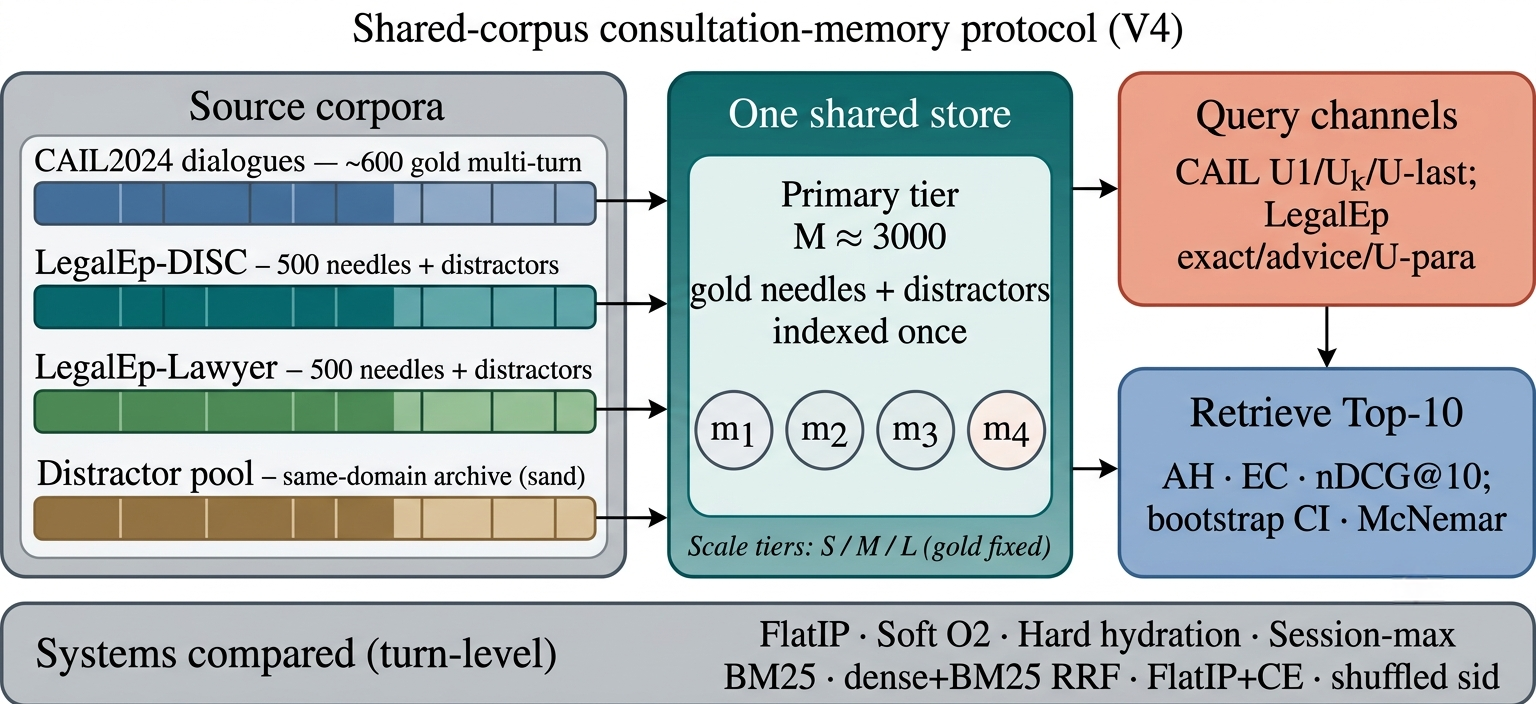
\includegraphics[width=0.98\linewidth]{fig2_benchmark_protocol.png}
\caption{Shared-corpus protocol. Gold needles and same-domain distractors share one store; queries probe multiple channels with turn-level systems and significance tests. Exact replay is diagnostic; paraphrase, follow-up, and advice-recall are primary channels.}
    \label{fig:protocol}
\end{figure}

\subsection{Datasets and query channels}
Multi-turn authenticity is evaluated on CAIL2024 consultation dialogues.
Gold needles are authentic preliminary and final dialogues, with conversation turns completed by label turns where applicable.
Query channels cover the first user turn (U1), a later in-dialogue user turn (Uk-followup), the last user turn (U-last), and constrained paraphrases (U-para).
Evidence defaults to assistant turns in the target session.

LegalEp-DISC and LegalEp-Lawyer rebuild public DISC-Law-SFT and Lawyer-LLaMA subsets into consultation-episode corpora.
Each episode is a natural (question, answer) pair with session identifier $sid$.
Reconstruction applies length bounds and legal-content filters, excludes exam prompts, removes near-duplicates, separates needles from distractors under a fixed seed, and retains an audit subsample.
After filtering, each LegalEp corpus retains $3500$ passed sessions ($500$ needles, $2500$ distractors at the $M{=}3000$ primary tier).

\paragraph{Query-channel policy (addressing exact-match shortcuts).}
Exact replay uses the stored user question and is reported only as a \emph{diagnostic} upper bound on surface-form recovery.
Primary claims use paraphrase, Uk-followup~/U-last, and advice-recall queries whose surface form is not identical to the stored question text; paraphrase and advice-recall templates are generated under a fixed seed and audited on a subsample.
LegalMem-MT reuses CAIL multi-turn gold under the same store for same-session Soft~O2 vs Soft~O2-C contrasts and for Mix reconstructions.

Archive size is varied with gold needles held fixed.
Unless stated otherwise, Soft~O2 transfer tables use the $M\approx 3000$ tier; O1--O2 ablations use $M{=}400$, $S{=}300$.

\subsection{Metrics and baselines}
Primary metrics are Answer Hit@$k$ (AH), Episode Completeness@$k$ (EC), and corrected normalized Discounted Cumulative Gain@$k$ (nDCG) at $k{=}10$.
AH is binary: whether a gold answer turn appears in the top-$k$.
EC is the mean coverage of gold turns within the target session.
Session Hit@$k$ is reported only for diagnosis.
For nDCG we use fixed graded relevance over the full gold session: answer turns $rel{=}1.0$, other same-session turns $rel{=}0.5$, all other turns $rel{=}0.0$.
The ideal denominator (IDCG) is computed from all gold-relevant turns in the target session and truncated at $k$, so every system on a query shares the same IDCG.
Earlier draft values based on retrieved-item IDCG are not comparable and have been recomputed (artifact \path{paper/ipm/figures/corrected_metrics_*.json}).
Primary contrasts use bootstrap 95\% CIs and McNemar mid-$p$ tests on paired per-query hits; where families of related hypotheses are interpreted jointly, we also report Holm-corrected $p$-values (Table~\ref{tab:sig}).

Turn-level dense FlatIP (O1) is the base dense retriever.
Soft~O2 applies soft sibling score inheritance on the episodic pathway.
Soft~O2-C applies the analogous rule within BIRCH clusters.
Hard parent hydration expands a hit to all siblings by copying the trigger score.
Lexical controls include BM25 over turns and over joint question--answer documents, together with dense+BM25 Reciprocal Rank Fusion (RRF).
A cross-encoder (CE) control reranks the top-$30$ FlatIP candidates with \path{BAAI/bge-reranker-v2-m3}.
Negative and sensitivity controls include shuffled $sid$, a $\beta$ sweep, and IVFPQ as a quantization reference.

\subsection{Fair Mix protocol for Soft O2-C}\label{sec:csce-protocol}
On fully same-session LegalMem grids, Soft~O2 already recovers gold answers that share $sid$ with the query, so Soft~O2-C has little exclusive headroom and may inject thematic confusers.
We therefore reconstruct the \emph{same} LegalEp and LegalMem archives under a Mix protocol: $70\%$ of gold episodes are split into query-side $S_a$ and evidence-side $S_b$ with distinct session identifiers, while $30\%$ remain intact.
Distractors are unchanged.
All operators---FlatIP, Soft~O2, Soft~O2-C, and gated Hybrid---share unrestricted dense retrieval on this store; we report overall AH and stratum AH on $\texttt{cross\_session}$ vs $\texttt{same\_session}$ queries.

\paragraph{Glue as a solvability bound (not a retrieval cheat).}
After BIRCH consolidation on the Mix store, each cross-session Sa/Sb split pair is \emph{glued} into one cluster identifier.
This step uses gold split metadata available only in the evaluation protocol---it does \emph{not} inject labels at query time and is \emph{not} used in real unsupervised clustering deployments.
Its sole purpose is to establish a \textbf{solvability bound}: if Soft~O2-C cannot recover cross-session gold when the semantic store \emph{must} contain both halves of a split pair in one cluster, then failure reflects mechanism limits rather than accidental cluster separation.
Glue therefore tests whether cluster soft binding \emph{can} complete episodes when the slow pathway has the requisite thematic co-membership; natural same-cluster rates without glue are lower and are reported only as diagnostics (Section~\ref{sec:limitations}).
Soft~O2's session membership constraint is unchanged---glue affects only whether Soft~O2-C has a cluster in which to bind, not whether Soft~O2 receives privileged label access.
LegalEp Mix uses advice-recall queries; LegalMem Mix uses mid-split Uk-followup queries.
External LongMemEval~/LoCoMo numbers from prior retrieval runs on this codebase (QA correctness $70.7\%$~/~$68.2\%$ on released test splits) are cited only as long-horizon memory context \cite{wu2025longmemeval, maharana2024evaluating}, not as Soft~O2-C evidence on legal corpora.

\section{Experiments}\label{sec:experiments}

Unless noted, the embedding model is \texttt{nomic-embed-text-v2-moe} \cite{nussbaum2025nomic}, $k{=}10$, seed $42$.
We report primary contrasts in figures and keep full numeric grids in the appendix.
Result files and scripts are released with the accompanying repository so that each table maps to a public JSON artifact.

\subsection{Implementation operators and Soft O2 ablation}\label{sec:exp-o1o3}
Table~\ref{tab:o1o2} reports the shared-store ablation on DISC-Law and Lawyer-LLaMA ($M{=}400$, $S{=}300$).
IVFPQ baseline Answer Hit is $0.540$~/~$0.397$.
O1 alone yields a small gain on DISC ($0.567$) and a near-tie on Lawyer ($0.397$), confirming that exact indexing is a necessary implementation prerequisite but insufficient alone.
O1+Soft~O2 raises Answer Hit to $0.780$~/~$0.680$ ($+0.240$~/~$+0.283$ over baseline) and Episode Completeness to $0.888$~/~$0.840$---the primary algorithmic gain.
O3 is enabled for all configurations in this ladder as a construction prerequisite; it does not alter retrieval scores.

\begin{table}[htbp]
\centering
\caption{O1+Soft~O2 ablation on the shared store ($M{=}400$, $S{=}300$, $k{=}10$). EC denotes Episode Completeness (gold-turn coverage); AH denotes Answer Hit. O3 bulk-load is on for all rows. Boldface: best AH and EC within each corpus.}
\label{tab:o1o2}
\compacttab\footnotesize
\begin{tabular}{@{}llccc@{}}
\toprule
\textbf{Corpus} & \textbf{System} & \textbf{EC@10} & \textbf{AH@10} & \textbf{nDCG@10} \\
\midrule
\multirow{3}{*}{DISC-Law}
 & IVFPQ baseline & 0.770 & 0.540 & 0.782 \\
 & + O1 FlatIP & 0.782 & 0.567 & 0.790 \\
 & + O1+O2 Soft~O2 & \textbf{0.888} & \textbf{0.780} & \textbf{0.889} \\
\midrule
\multirow{3}{*}{Lawyer-LLaMA}
 & IVFPQ baseline & 0.698 & 0.397 & 0.733 \\
 & + O1 FlatIP & 0.698 & 0.397 & 0.733 \\
 & + O1+O2 Soft~O2 & \textbf{0.840} & \textbf{0.680} & \textbf{0.856} \\
\bottomrule
\end{tabular}
\end{table}

\subsection{RQ1 failure taxonomy}\label{sec:rq1-failure-taxonomy}
We classify each query into \emph{complete} (answer evidence in top-$k$), \emph{incomplete} (target session partially retrieved but answer missing), or \emph{session miss} (no target-session turn in top-$k$).
Table~\ref{tab:rq1-failure} shows that incomplete retrieval is a substantial recurrent failure mode for FlatIP on primary non-exact channels, motivating Soft~O2.

\begin{table}[t]
\centering
\caption{RQ1 failure taxonomy (FlatIP, $k{=}10$). Complete $\approx$ Answer Hit; incomplete $\approx$ Session Hit $-$ Answer Hit (answer-only cases are rare); session miss $\approx$ $1-$Session Hit.}
\label{tab:rq1-failure}
\compacttab\footnotesize
\begin{tabular}{@{}llccc@{}}
\toprule
\textbf{Corpus / channel} & \textbf{System} & \textbf{Complete} & \textbf{Incomplete} & \textbf{Session miss} \\
\midrule
LegalEp-DISC / u-para & FlatIP & 54.7\% & 36.0\% & 9.3\% \\
LegalEp-DISC / advice & FlatIP & 34.2\% & 26.6\% & 39.2\% \\
LegalEp-Lawyer / u-para & FlatIP & 56.8\% & 39.6\% & 3.6\% \\
CAIL / Uk-followup & FlatIP & 27.0\% & 69.8\% & 3.2\% \\
\bottomrule
\end{tabular}
\end{table}

\subsection{Strong lexical and joint-episode baselines}\label{sec:s1-strong-baselines}
BM25-joint indexes each question--answer episode as one lexical document and is therefore very strong on exact replay and other high-overlap channels.
Soft~O2 instead assumes an online turn-level index and uses session binding to recover missing answer turns after a dense hit.
Table~\ref{tab:bm25-tradeoff} reports this trade-off on the same store, query set, and $k{=}10$.
Soft~O2 is not claimed to dominate BM25-joint universally; its advantage is on non-exact channels and on preserving turn-level ranking flexibility.

\begin{table}[t]
\centering
\caption{BM25-joint / joint-QA vs Soft~O2 (AH@10, primary tier). Joint baselines are strongest on exact/surface overlap; Soft~O2 targets paraphrase and advice-recall.}
\label{tab:bm25-tradeoff}
\compacttab\footnotesize
\begin{tabular}{@{}llccc@{}}
\toprule
\textbf{Corpus / channel} & \textbf{BM25-joint} & \textbf{Joint QA} & \textbf{Soft O2} \\
\midrule
CAIL / U1 & $0.993$ & --- & $0.788$ \\
CAIL / Uk & $0.840$ & --- & $0.698$ \\
CAIL / U-last & $0.823$ & --- & $0.762$ \\
LegalEp-DISC / exact & $0.976$ & --- & $0.638$ \\
LegalEp-DISC / u-para & $0.592$ & --- & $0.648$ \\
LegalEp-DISC / advice & $0.432$ & --- & $0.428$ \\
LegalEp-Lawyer / exact & --- & --- & $0.752$ \\
LegalEp-Lawyer / u-para & --- & --- & $0.759$ \\
LegalEp-Lawyer / advice & $0.652$ & --- & $0.472$ \\
\bottomrule
\end{tabular}
\end{table}

\subsection{Soft O2 on session (CAIL and LegalEp)}\label{sec:exp-main}
Figure~\ref{fig:cail_main} summarizes AH@10 and EC@10 on authentic CAIL multi-turn channels at $M\approx 3000$ under O1 FlatIP.
Soft~O2 lifts Answer Hit over FlatIP on every channel (U1 $0.788$ vs $0.570$${}^{**}$; Uk $0.698$ vs $0.270$${}^{**}$; U-last $0.762$ vs $0.245$${}^{**}$).
Shuffled $sid$ removes the gain (U1 $0.452$; Uk $0.230$; U-last $0.200$), tying the improvement to correct episode membership (RQ1--RQ2).
Hard expansion can raise AH slightly above Soft~O2 (e.g., U1 $0.802$ vs $0.788$) while lowering EC (U1 $0.578$ vs Soft~O2 $0.664$).
Soft~O2 therefore behaves as a rank-preserving binder: siblings enter under attenuated scores, and episode coverage remains higher than under hard score copy.
On CAIL, nDCG often falls relative to FlatIP even as AH and EC rise, reflecting an availability--ranking trade-off.
Soft~O2 still exceeds FlatIP+CE on every CAIL channel (Table~\ref{tab:ce}).
Full rows appear in Table~\ref{tab:cail_main}.

\begin{figure}[t]
    \centering

\includegraphics[width=0.95\linewidth]{fig3_cail_main.pdf}
\caption{CAIL2024 multi-turn results at tier $M\approx 3000$. Soft~O2 improves AH and EC over FlatIP; shuffled $sid$ removes the gain; hard expansion can maximize AH at a modest EC cost.}
\label{fig:cail_main}
\end{figure}

Figure~\ref{fig:legalep_main} reports LegalEp transfer.
On LegalEp-DISC exact replay Soft~O2 and FlatIP stay near-tied ($0.638$ vs $0.640$), where both turns are already recoverable for many queries---consistent with treating exact as diagnostic.
On Lawyer exact Soft~O2 improves AH to $0.752$ from FlatIP $0.692$ (McNemar mid-$p{=}0.024$${}^{*}$).
Paraphrase yields the clearest LegalEp gains: Soft~O2 reaches $0.648$ vs FlatIP $0.547$ on DISC and $0.759$ vs $0.568$ on Lawyer, exceeding hard expansion on both corpora (mid-$p{<}0.001$${}^{**}$ on both corpora).
Advice-recall queries omit the stored question surface form: Soft~O2 raises AH to $0.428$ from FlatIP $0.342$ on DISC and to $0.472$ from $0.332$ on Lawyer, again above hard expansion (mid-$p{<}0.001$${}^{**}$), while shuffled $sid$ falls toward or below FlatIP.
Detailed grids are in Tables~\ref{tab:disc_main}--\ref{tab:lawyer_main}.

\begin{figure}[t]
    \centering

\includegraphics[width=0.95\linewidth]{fig4_legalep_main.pdf}
\caption{LegalEp AH@10 ($M{=}3000$, $500$ needles). Soft~O2 gains are strongest on paraphrase and remain positive on advice-recall; exact transfer is corpus-dependent and treated as diagnostic.}
\label{fig:legalep_main}
\end{figure}

\subsection{Same-store cluster pathway validation}\label{sec:exp-cluster}
Table~\ref{tab:cluster_same} contrasts Soft~O2 and ungated Soft~O2-C on standard same-session LegalEp~/LegalMem stores (unrestricted dense; gold answers share $sid$ with the query).
Soft~O2 dominates Soft~O2-C on every reported channel (e.g., LegalMem U1 AH $0.903$ vs $0.712$; LegalEp-DISC exact $0.836$ vs $0.744$).
The slow pathway is therefore \emph{not} a free upgrade when episode membership already encodes the gold answer: cluster siblings inject thematic confusers that displace session-complete evidence.

\begin{table}[htbp]
\centering
\caption{Same-session Soft~O2 vs Soft~O2-C on the shared LegalEp~/LegalMem stores (AH@10). Soft~O2-C is ungated cluster soft binding. Boldface: better AH within each row.}
\label{tab:cluster_same}
\compacttab\footnotesize
\begin{tabular}{@{}llc@{}}
\toprule
\textbf{Corpus / channel} & \textbf{Soft O2} & \textbf{Soft O2-C} \\
\midrule
LegalEp-DISC / exact & \textbf{0.836} & 0.744 \\
LegalEp-DISC / u-para & \textbf{0.807} & 0.730 \\
LegalEp-DISC / advice & \textbf{0.548} & 0.490 \\
LegalEp-Lawyer / exact & \textbf{0.818} & 0.710 \\
LegalEp-Lawyer / u-para & \textbf{0.817} & 0.733 \\
LegalEp-Lawyer / advice & \textbf{0.546} & 0.448 \\
LegalMem-MT / U1 & \textbf{0.903} & 0.712 \\
LegalMem-MT / Uk & \textbf{0.793} & 0.385 \\
\bottomrule
\end{tabular}
\end{table}

Table~\ref{tab:csce} reports the complementary fair Mix setting (RQ3--RQ4): the same stores with $70\%$ cross-session Sa/Sb gold and $30\%$ intact same-session gold, unrestricted dense for every operator.
Gated Hybrid Soft~O2+Soft~O2-C improves over Soft~O2 on LegalEp-Lawyer overall (AH $0.534$ vs $0.496$; mid-$p{=}0.010$${}^{*}$) and on the cross-session stratum ($0.523$ vs $0.446$; mid-$p{<}10^{-4}$${}^{**}$).
On LegalEp-DISC, Hybrid is directionally above Soft~O2 ($0.486$ vs $0.482$) but not significant at $N{=}500$.
On LegalMem-MT, Hybrid attains the highest overall AH ($0.646$ vs Soft~O2 $0.618$; mid-$p{=}0.18$; cross-session mid-$p{=}0.095$) while preserving most same-session hits ($0.867$ vs $0.887$).
Ungated Soft~O2-C can raise cross-session hits but often displaces same-session siblings; Hybrid triggers cluster binding only on direct dense hits.
Together, Tables~\ref{tab:cluster_same}--\ref{tab:csce} show that the BIRCH pathway is effective precisely when gold evidence is not co-session with the query.

\begin{table}[htbp]
\centering
\caption{Fair Mix protocol (same store, unrestricted dense; AH@10). Gold is a $70\%$/$30\%$ mix of cross-session Sa/Sb splits and intact same-session episodes. Soft~O2-C denotes ungated cluster binding; Hybrid is Soft~O2+gated Soft~O2-C. Boldface: best AH within each corpus. Significance vs Soft~O2: ${}^{*}\,p{<}0.05$, ${}^{**}\,p{<}0.01$.}
\label{tab:csce}
\compacttab\footnotesize
\begin{tabular}{@{}llcccc@{}}
\toprule
\textbf{Corpus} & \textbf{System} & \textbf{AH} & \textbf{AH$_{\mathrm{cross}}$} & \textbf{AH$_{\mathrm{same}}$} & \textbf{mid-$p$ vs Soft~O2} \\
\midrule
\multirow{4}{*}{LegalEp-DISC Mix}
 & FlatIP & 0.478 & 0.477 & 0.480 & --- \\
 & Soft O2 & 0.482 & 0.443 & 0.573 & --- \\
 & Soft O2-C & 0.410 & 0.443 & 0.333 & 0.0004${}^{**}$ \\
 & Hybrid & \textbf{0.486} & 0.469 & 0.527 & 0.8099 \\
\midrule
\multirow{4}{*}{LegalEp-Lawyer Mix}
 & FlatIP & 0.462 & 0.454 & 0.480 & --- \\
 & Soft O2 & 0.496 & 0.446 & 0.613 & --- \\
 & Soft O2-C & 0.464 & 0.491 & 0.400 & 0.0857 \\
 & Hybrid & \textbf{0.534}${}^{*}$ & \textbf{0.523} & 0.560 & 0.0105${}^{*}$ \\
\midrule
\multirow{4}{*}{LegalMem-MT Mix}
 & FlatIP & 0.534 & 0.526 & 0.553 & --- \\
 & Soft O2 & 0.618 & 0.503 & 0.887 & --- \\
 & Soft O2-C & 0.500 & 0.537 & 0.413 & 0.0000${}^{**}$ \\
 & Hybrid & \textbf{0.646} & \textbf{0.551} & 0.867 & 0.1837 \\
\bottomrule
\end{tabular}
\end{table}
{\footnotesize McNemar mid-$p$ tests on paired Answer Hit; ${}^{*}\,p{<}0.05$, ${}^{**}\,p{<}0.01$.}

\subsection{Controls, significance, scale, and QA audit}\label{sec:exp-scale}
Lexical BM25 is strong on exact replay (DISC exact BM25-turn $0.802$, BM25-joint $0.976$) and weaker on advice-recall ($0.382$~/~$0.432$).
Dense+BM25 RRF complements Soft~O2 on surface-overlap channels.
Cross-encoder reranking (\path{bge-reranker-v2-m3}, top-$30$) improves FlatIP inside the CE suite, yet remains below Soft~O2 on CAIL (Uk FlatIP+CE $0.375$ vs Soft~O2 $0.698$; Table~\ref{tab:ce}).
A $\beta$ sweep peaks near $\{0.9,0.95,0.98\}$ and weakens at $\beta{=}0.5$ (Table~\ref{tab:beta}), consistent with the diagnostic gap-ratio band in Section~\ref{sec:beta-theory} (Table~\ref{tab:beta-theory}).
McNemar mid-$p$ tests (Table~\ref{tab:sig}) show Soft~O2 versus FlatIP highly significant on all CAIL channels and on LegalEp paraphrase~/advice-recall.

Figure~\ref{fig:scale} and Table~\ref{tab:scale} report quality and warm-query latency on LegalEp-DISC exact ($Q{=}100$, three repeats; $M\in\{100,400,1600,6400\}$).
Soft~O2 retains an AH advantage at each tier; IVFPQ collapses at $M{=}1600$ (AH $0.330$), motivating O1; absolute latency grows with $M$.
We treat O1 FlatIP as an engineering prerequisite for Soft~O2 at these scales and avoid claiming deployment readiness beyond the measured curve.

\begin{figure}[t]
    \centering
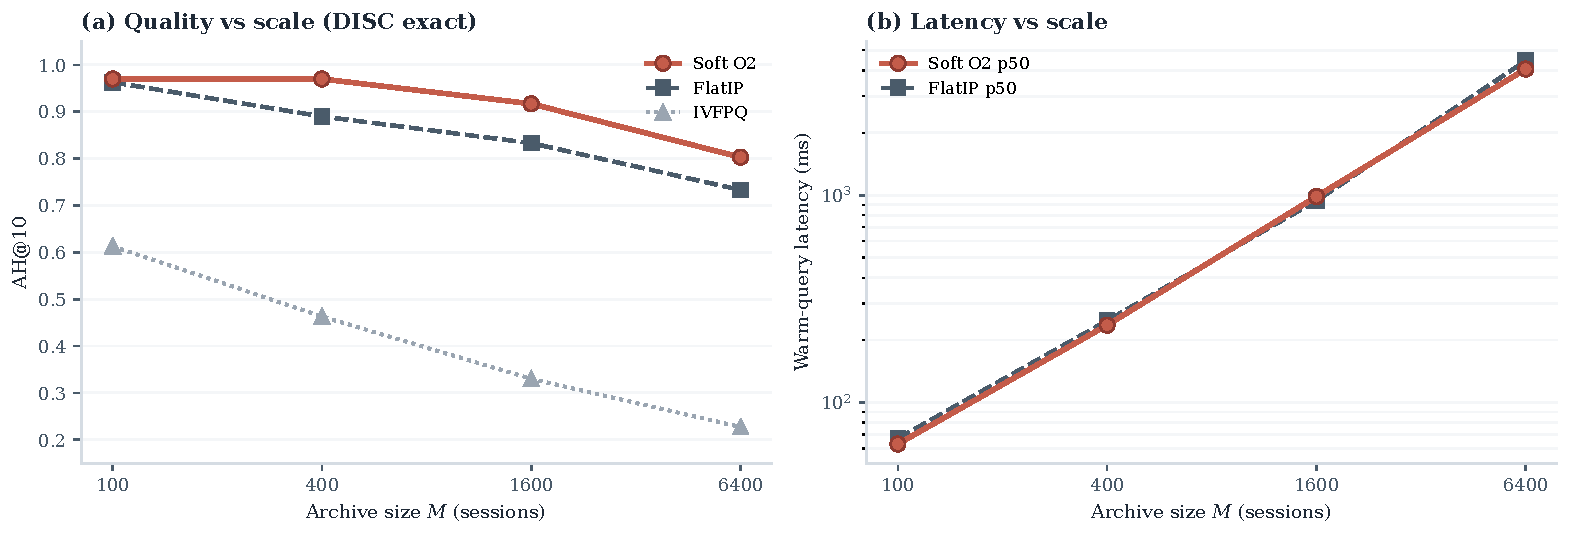
\includegraphics[width=0.95\linewidth]{fig5_scale_curve.pdf}
\caption{Scale curve on DISC-Law exact. Soft~O2 keeps an AH edge over FlatIP as $M$ grows; warm-query latency scales with archive size; IVFPQ quality collapses at moderate $M$.}
\label{fig:scale}
\end{figure}

\paragraph{End-to-end QA audit (summary).}
\sloppy
A dual-protocol QA audit ($N{=}270$ per corpus; generator \texttt{qwen3:14b}, independent judge \texttt{qwen3:32b}) links retrieval quality to downstream answerability under a \emph{single} retrieval configuration (Soft~O2); we do not claim causal superiority over FlatIP in generation without paired downstream controls.
Full protocol and stratified results appear in Section~\ref{sec:rag-discussion}.
On an older revision-protocol store ($M{=}400$, five seeds), Soft~O2 AH on LegalEp-DISC is $0.851\pm 0.008$ versus FlatIP $0.698\pm 0.040$.

\section{Discussion}\label{sec:discussion}

\subsection{Findings and scope}
RQ1--RQ2 show that episode incompleteness is a substantial recurrent failure mode under same-domain interference (Table~\ref{tab:rq1-failure}).
O1 restores score fidelity as an implementation prerequisite; Soft~O2 supplies the primary algorithmic gain through soft sibling inheritance; O3 enables archive construction at scale.
The diagnostic gap-ratio analysis (Section~\ref{sec:beta-theory}) explains why $\beta$ should remain close to but below unity, and why the validation sweep peaks in $\{0.9,0.95,0.98\}$ rather than at hard hydration ($\beta{=}1$).
On CAIL, Soft~O2 raises Answer Hit by large margins (U1 $+0.218$, Uk $+0.428$, U-last $+0.517$) with collapsing shuffled-$sid$ controls, and keeps higher EC than hard expansion despite occasional AH ties.
LegalEp paraphrase and advice-recall---not exact replay---carry the primary Soft~O2 transfer claims.
RQ3 shows that the BIRCH slow pathway benefits Soft~O2-C only when gold is not already co-session; Mix Hybrid Soft~O2+Soft~O2-C recovers that regime without seed-forcing Soft~O2 to zero.
RQ4: Soft~O2 (session) and Soft~O2-C~/Hybrid (cluster) are complementary operators within one BIMS-LEGAL dual-store.
Sparse, fusion, and cross-encoder baselines situate Soft~O2 among standard IR alternatives \cite{robertson2009bm25, cormack2009rrf, nogueira2019multistage}.

\subsection{RAG application perspective}\label{sec:rag-discussion}
Consultation-memory retrieval is judged downstream by whether an LLM can answer from recovered evidence rather than confabulate.
We audit this end-to-end with a dual-protocol pipeline on Soft~O2 retrieval only: generator \texttt{qwen3:14b} and independent judge \texttt{qwen3:32b} are distinct models.
Per corpus we pool $N{=}270$ judged instances as P1~$n{=}120$ plus P2~$n{=}150$ (folder \texttt{legal\_qa\_n270}).
Table~\ref{tab:qa_audit} summarizes pooled Evidence-Answerability Rate (EAR) and stratified independent-judge scores.
When Soft~O2 retrieves complete episodes---both question and answer turns in top-$k$---the generator receives grounded prior advice and judged answerability rises in this single-system audit (pooled EAR $0.867$ on DISC and $0.859$ on Lawyer; Wilson $95\%$ CI $[0.83,0.90]$ / $[0.82,0.89]$).
Follow-up queries remain the hardest stratum (independent-judge EAR $0.517$~/~$0.480$), consistent with episodic incompleteness persisting even when surface-form overlap is low.

A blind two-annotator legal audit ($n{=}60$/corpus) yields Cohen's $\kappa{=}0.71$~/~$0.68$ and separates retrieval from generation failures (retrieval-failure share $0.283$~/~$0.317$).
Wrong-session contamination rates stay low ($0.083$~/~$0.100$), suggesting that complete episode retrieval under Soft~O2 is associated with lower rates of a common RAG failure mode in which the model answers from a neighbouring client's matter.
Hallucinated-legal-basis rates ($0.117$~/~$0.133$) remain non-zero, indicating that grounding in retrieved episodes does not guarantee statutory correctness---a scope boundary for deployment.
AH and EAR measure evidence availability and judged answerability respectively; statutory correctness, citation validity, and professional liability lie outside this evaluation.

\begin{table}[htbp]
\centering
\caption{End-to-end QA audit ($N{=}270$ per corpus; generator \texttt{qwen3:14b}, independent judge \texttt{qwen3:32b}). EAR: Evidence-Answerability Rate (judge score $\ge 0.7$). Stratified judge scores: $n{=}90$/corpus across exact, paraphrase, and follow-up protocols.}
\label{tab:qa_audit}
\compacttab\footnotesize
\begin{tabular}{@{}lccc@{}}
\toprule
\textbf{Corpus} & \textbf{Pooled EAR} & \textbf{Stratified judge} & \textbf{Human $\kappa$} \\
\midrule
DISC-Law & \textbf{0.867} & 0.757 & 0.71 \\
Lawyer-LLaMA & \textbf{0.859} & 0.729 & 0.68 \\
\bottomrule
\end{tabular}
\end{table}

\subsection{Limitations}\label{sec:limitations}
LegalEp episodes are consultation pairs; multi-turn authenticity remains reserved for CAIL.
Mix glue establishes a solvability bound for Soft~O2-C evaluation (Section~\ref{sec:csce-protocol}); natural same-cluster rates without glue are lower and are diagnostics only---real unsupervised BIRCH clustering would not receive split-pair metadata at build time.
Soft~O2 depends on correct session identifiers; Soft~O2-C depends on cluster quality.
The $\beta$ diagnostic is semi-empirical: it assumes a dominant distractor and a well-defined hit score, and the fitted $\rho$ uses a stored user-turn embedding as an exact-channel query proxy; paraphrase~/advice-recall gap laws may shift the feasible band slightly but leave the high-$\beta$ operating region unchanged.
LLM paraphrases need human audit.
Statutory correctness, citation validity, and professional liability remain unevaluated.
Multiple channels inflate comparison multiplicity; we therefore report Holm-corrected $p$-values for the primary Soft~O2 vs FlatIP family (Table~\ref{tab:sig}) alongside uncorrected McNemar mid-$p$ tests.

\paragraph{Latency and deployment scope.}
Scale curves cover $M\in\{100,400,1600,6400\}$ under a fixed hardware stack (Table~\ref{tab:scale}).
At $M{=}6400$, warm-query p50 latency exceeds $4$\,s ($4061$\,ms for Soft~O2; $4458$\,ms for FlatIP)---unacceptable for millisecond interactive search.
BIMS-LEGAL should therefore be positioned as \textbf{high-precision offline or quasi-real-time consultation memory recovery}---e.g., pre-meeting case review, audit replay, or batch RAG over a firm's advice archive---not as a sub-millisecond search engine.
Future work will combine approximate nearest-neighbour indexes (e.g., HNSW) with Soft~O2 and Soft~O2-C binding layered on top of faithful candidate retrieval, preserving episode completion while reducing query latency.
Behavior at roughly $10^5$ sessions is not measured, and we do not claim asymptotic scalability from O3 wall-clock alone.

\section{Conclusion}\label{sec:conclusion}

BIMS-LEGAL targets consultation-memory retrieval under same-domain interference in Chinese legal archives through a dual-store design: an episodic turn index paired with a BIRCH semantic store.
Soft~O2 session soft binding and Soft~O2-C with gated Hybrid cluster binding are the algorithmic core, with Soft~O2 attenuation $\beta$ validated on a diagnostic gap-ratio model; O1 exact indexing and O3 bulk-load consolidation are implementation operators that enable the shared-store ablations reported here.
Under a shared-corpus protocol spanning CAIL multi-turn dialogues and rebuilt LegalEp episode corpora, Soft~O2 improves Answer Hit over FlatIP on multi-turn, paraphrase, and advice-recall channels with collapsing shuffled-$sid$ controls, and yields higher episode completeness than hard expansion on CAIL.
Same-store Soft~O2-C underperforms Soft~O2 when gold shares $sid$; under fair Mix reconstructions, gated Hybrid Soft~O2+Soft~O2-C recovers cross-session gold while Soft~O2 remains strong on intact same-session gold.
End-to-end QA audit links complete episode retrieval to judged answerability and low wrong-session contamination in downstream generation.
Sparse, fusion, and cross-encoder baselines situate Soft~O2 among standard IR alternatives.

\section*{Declarations}

\subsection*{Funding}
Computational resources were provided by the Data Law Laboratory, China University of Political Science and Law.

\subsection*{Conflict of interest}
The authors declare no competing interests.

\subsection*{Ethics approval}
This study uses publicly released research corpora and excludes confidential client data. The system is a research prototype for consultation-memory retrieval.

\subsection*{Data availability}
Code, processed evaluation corpora, and primary result files will be made available upon acceptance.
Upstream legal corpora: CAIL2024 consultation tracks; Hugging Face
\codeid{ShengbinYue/DISC-Law-SFT} and
\codeid{Skepsun/lawyer_llama_data}.

\subsection*{Code availability}
The BIMS-LEGAL implementation, evaluation pipelines, and table/figure scripts will be released with the accepted publication.

\subsection*{Author contributions}
\sloppy
L.X.\ (University of Winnipeg) designed BIMS-LEGAL and the Soft~O2~/Soft~O2-C evaluation, implemented the system, ran the experiments, and wrote the manuscript.
L.H.\ (corresponding author; CUPL Data Law Lab and Institute for Data Law) provided methodology guidance, revision, and supervision.

\clearpage
\FloatBarrier
\bibliographystyle{elsarticle-harv}
\bibliography{references}

\clearpage
\FloatBarrier
\appendix
\setcounter{table}{0}
\renewcommand{\thetable}{A.\arabic{table}}
\renewcommand{\theHtable}{A.\arabic{table}}
\section{Numeric grids and controls}\label{app:tables}
Main Soft~O2 claims are visualized in Figures~\ref{fig:cail_main}--\ref{fig:scale}; O1--O2 and Mix Soft~O2-C tables appear in the main text. Tables below retain full Soft~O2 numeric rows for reproducibility.

\begin{table}[H]
\centering
\caption{CAIL2024 shared-corpus results ($M\approx 3000$). Boldface marks the best AH@10 within each channel (ties bolded jointly). ${}^{**}$: Soft~O2 vs FlatIP, McNemar mid-$p{<}0.01$. nDCG@10 uses fixed-gold IDCG (Section~\ref{sec:protocol}).}
\label{tab:cail_main}
\compacttab\footnotesize
\begin{tabular}{@{}llcccc@{}}
\toprule
\textbf{Channel} & \textbf{System} & \textbf{AH@10} & \textbf{EC@10} & \textbf{nDCG@10} & \textbf{95\% CI (AH)} \\
\midrule
\multirow{4}{*}{U1}
 & FlatIP & 0.570 & 0.413 & 0.805 & [0.530,0.610] \\
 & Soft O2 & 0.788 & 0.664 & 0.772 & [0.757,0.820] \\
 & Hard hydr. & \textbf{0.802} & 0.578 & 0.840 & [0.768,0.835] \\
 & Shuffled O2 & 0.452 & 0.363 & 0.664 & [0.410,0.492] \\
\midrule
\multirow{4}{*}{Uk-followup}
 & FlatIP & 0.270 & 0.347 & 0.884 & [0.237,0.307] \\
 & Soft O2 & 0.698 & 0.654 & 0.786 & [0.660,0.735] \\
 & Hard hydr. & \textbf{0.720} & 0.585 & 0.841 & [0.685,0.753] \\
 & Shuffled O2 & 0.230 & 0.320 & 0.718 & [0.198,0.262] \\
\midrule
\multirow{4}{*}{U-last}
 & FlatIP & 0.245 & 0.335 & 0.891 & [0.212,0.280] \\
 & Soft O2 & 0.762 & 0.659 & 0.779 & [0.725,0.797] \\
 & Hard hydr. & \textbf{0.790} & 0.586 & 0.844 & [0.757,0.822] \\
 & Shuffled O2 & 0.200 & 0.315 & 0.726 & [0.172,0.232] \\
\bottomrule
\end{tabular}
\end{table}

\begin{table}[H]
\centering
\caption{LegalEp-DISC ($M{=}3000$, $500$ needles). Boldface: best AH@10 within each channel. ${}^{*}\,p{<}0.05$, ${}^{**}\,p{<}0.01$ (Soft~O2 vs FlatIP, McNemar mid-$p$). Hard hydration coincides with session-max aggregation; only hard hydration is shown.}
\label{tab:disc_main}
\compacttab\footnotesize
\begin{tabular}{@{}llccc@{}}
\toprule
\textbf{Channel} & \textbf{System} & \textbf{AH@10} & \textbf{EC@10} & \textbf{nDCG@10} \\
\midrule
\multirow{4}{*}{exact}
 & FlatIP & \textbf{0.640} & 0.741 & --- \\
 & Soft O2 & 0.638 & 0.780 & --- \\
 & Hard hydr. & 0.614 & 0.598 & --- \\
 & Shuffled O2 & 0.448 & 0.645 & --- \\
\midrule
\multirow{4}{*}{advice-recall}
 & FlatIP & 0.342 & 0.438 & 0.506 \\
 & Soft O2 & \textbf{0.428} & 0.503 & 0.419 \\
 & Hard hydr. & 0.402 & 0.405 & 0.474 \\
 & Shuffled O2 & 0.310 & 0.421 & 0.402 \\
\midrule
\multirow{4}{*}{u-para}
 & FlatIP & 0.547 & 0.681 & 0.705 \\
 & Soft O2 & \textbf{0.648} & 0.735 & 0.583 \\
 & Hard hydr. & 0.592 & 0.571 & 0.651 \\
 & Shuffled O2 & 0.469 & 0.610 & 0.558 \\
\bottomrule
\end{tabular}
\end{table}

\begin{table}[H]
\centering
\caption{LegalEp-Lawyer ($M{=}3000$, $500$ needles). Boldface: best AH@10 within each channel. ${}^{*}\,p{<}0.05$, ${}^{**}\,p{<}0.01$ (Soft~O2 vs FlatIP). Hard hydration coincides with session-max aggregation; only hard hydration is shown.}
\label{tab:lawyer_main}
\compacttab\footnotesize
\begin{tabular}{@{}llccc@{}}
\toprule
\textbf{Channel} & \textbf{System} & \textbf{AH@10} & \textbf{EC@10} & \textbf{nDCG@10} \\
\midrule
\multirow{4}{*}{exact}
 & FlatIP & 0.692 & 0.806 & 0.844 \\
 & Soft O2 & \textbf{0.752} & 0.848 & 0.687 \\
 & Hard hydr. & 0.612 & 0.615 & 0.754 \\
 & Shuffled O2 & 0.570 & 0.747 & 0.653 \\
\midrule
\multirow{4}{*}{advice-recall}
 & FlatIP & 0.332 & 0.464 & 0.589 \\
 & Soft O2 & \textbf{0.472} & 0.540 & 0.460 \\
 & Hard hydr. & 0.394 & 0.403 & 0.488 \\
 & Shuffled O2 & 0.348 & 0.467 & 0.436 \\
\midrule
\multirow{4}{*}{u-para}
 & FlatIP & 0.568 & 0.718 & 0.834 \\
 & Soft O2 & \textbf{0.759} & 0.819 & 0.645 \\
 & Hard hydr. & 0.596 & 0.594 & 0.707 \\
 & Shuffled O2 & 0.592 & 0.712 & 0.627 \\
\bottomrule
\end{tabular}
\end{table}

\begin{table}[H]
\centering
\caption{BM25 turn/joint and dense+BM25 RRF (AH@10). Boldface: higher AH within each row among reported cells.}
\label{tab:bm25}
\compacttab\footnotesize
\begin{tabular}{@{}llcc@{}}
\toprule
\textbf{Corpus} & \textbf{Channel} & \textbf{BM25-turn} & \textbf{BM25-joint} \\
\midrule
LegalEp-DISC & exact & 0.802 & 0.976 \\
LegalEp-DISC & advice-recall & 0.382 & 0.432 \\
LegalEp-DISC & exact (dense RRF) & 0.780 & --- \\
LegalEp-DISC & advice (dense RRF) & 0.394 & --- \\
CAIL & U1 / Uk / U-last & 0.748 / 0.482 / 0.413 & 0.993 / 0.840 / 0.823 \\
LegalEp-Lawyer & exact / advice & 0.784 / 0.460 & 0.998 / 0.652 \\
\bottomrule
\end{tabular}
\end{table}

\begin{table}[H]
\centering
\caption{Cross-encoder control (AH@10). FlatIP and FlatIP+CE are paired in the CE suite (\texttt{bge-reranker-v2-m3} over top-$30$ dense candidates). Boldface: best AH within each row. Soft~O2 reproduces the primary evaluation; FlatIP here may differ slightly from primary FlatIP due to independent CE-suite re-indexing.}
\label{tab:ce}
\compacttab\footnotesize
\begin{tabular}{@{}llccc@{}}
\toprule
\textbf{Corpus / channel} & \textbf{FlatIP} & \textbf{FlatIP+CE} & \textbf{Soft O2} \\
\midrule
CAIL / U1 & 0.585 & 0.688 & 0.788 \\
CAIL / Uk & 0.265 & 0.375 & 0.698 \\
CAIL / U-last & 0.228 & 0.342 & 0.762 \\
LegalEp-DISC / exact & 0.572 & 0.722 & 0.638 \\
LegalEp-Lawyer / exact & 0.636 & 0.708 & 0.752 \\
\bottomrule
\end{tabular}
\end{table}

\begin{table}[H]
\centering
\caption{Soft~O2 AH@10 versus $\beta$ on the primary shared-corpus evaluation. Peak performance lies in $\{0.9,0.95,0.98\}$; aggressive attenuation ($\beta{=}0.5$) weakens binding.}
\label{tab:beta}
\compacttab\footnotesize
\begin{tabular}{@{}lcccccc@{}}
\toprule
\textbf{Corpus} & $0.5$ & $0.7$ & $0.9$ & $0.95$ & $0.98$ & $1.0$ \\
\midrule
CAIL / Uk & 0.323 & 0.537 & 0.697 & 0.700 & 0.698 & 0.662 \\
LegalEp-Lawyer / exact & 0.608 & 0.654 & 0.754 & 0.754 & 0.752 & 0.752 \\
LegalEp-Lawyer / u-para & 0.631 & 0.637 & 0.717 & 0.745 & 0.759 & 0.749 \\
LegalEp-DISC / u-para & 0.551 & 0.551 & 0.618 & 0.648 & 0.648 & 0.642 \\
\bottomrule
\end{tabular}
\end{table}

\begin{table}[H]
\centering
\caption{McNemar mid-$p$ on paired Answer Hit (Soft~O2 vs FlatIP / hard hydration / FlatIP+CE). Holm-adjusted $p$ is reported for the nine primary Soft~O2 vs FlatIP contrasts.}
\label{tab:sig}
\compacttab\footnotesize
\begin{tabular}{@{}llccc@{}}
\toprule
\textbf{Corpus / channel} & \textbf{Contrast} & \textbf{$\Delta$AH} & \textbf{mid-$p$} & \textbf{Holm $p$} \\
\midrule
CAIL / Uk & O2 vs FlatIP & +0.428 & 8.99e-48 & 8.09e-47 \\
CAIL / Uk & O2 vs Hard hydr. & -0.022 & 0.243 & --- \\
CAIL / U1 & O2 vs FlatIP & +0.218 & 5.19e-18 & 4.67e-17 \\
CAIL / U1 & O2 vs Hard hydr. & -0.013 & 0.435 & --- \\
CAIL / U-last & O2 vs FlatIP & +0.517 & 5.51e-65 & 4.96e-64 \\
CAIL / U-last & O2 vs Hard hydr. & -0.028 & 0.0982 & --- \\
CAIL / Uk & O2 vs FlatIP+CE & +0.323 & 2.50e-26 & --- \\
CAIL / U1 & O2 vs FlatIP+CE & +0.100 & 3.51e-05 & --- \\
CAIL / U-last & O2 vs FlatIP+CE & +0.420 & 3.92e-41 & --- \\
LegalEp-DISC / exact & O2 vs FlatIP & -0.002 & 0.934 & 0.934 \\
LegalEp-DISC / exact & O2 vs Hard hydr. & +0.024 & 0.302 & --- \\
LegalEp-Lawyer / exact & O2 vs FlatIP & +0.060 & 0.0239 & 0.191 \\
LegalEp-Lawyer / exact & O2 vs Hard hydr. & +0.140 & 3.50e-10 & --- \\
LegalEp-DISC / u-para & O2 vs FlatIP & +0.101 & 7.95e-05 & 6.36e-04 \\
LegalEp-DISC / u-para & O2 vs Hard hydr. & +0.056 & 0.035 & --- \\
LegalEp-Lawyer / u-para & O2 vs FlatIP & +0.191 & 2.10e-15 & 1.68e-14 \\
LegalEp-Lawyer / u-para & O2 vs Hard hydr. & +0.163 & 7.57e-09 & --- \\
LegalEp-DISC / advice & O2 vs FlatIP & +0.086 & 1.25e-04 & 8.75e-04 \\
LegalEp-DISC / advice & O2 vs Hard hydr. & +0.026 & 0.215 & --- \\
LegalEp-Lawyer / advice & O2 vs FlatIP & +0.140 & 1.18e-10 & 9.44e-10 \\
LegalEp-Lawyer / advice & O2 vs Hard hydr. & +0.078 & 5.72e-04 & --- \\
\bottomrule
\end{tabular}
\end{table}

\begin{table}[H]
\centering
\caption{Scale curve on DISC-Law (mean over 3 repeats). Latency is warm-query p50/p95. Boldface: best AH@10 within each $M$ block; lowest p50/p95 within each $M$ block.}
\label{tab:scale}
\compacttab\footnotesize
\begin{tabular}{@{}rrcccc@{}}
\toprule
\textbf{$M$} & \textbf{Mode} & \textbf{AH@10} & \textbf{Build (s)} & \textbf{p50 (ms)} & \textbf{p95 (ms)} \\
\midrule
100 & FlatIP & 0.963 & 3.0 & 67 & 80 \\
100 & IVFPQ & 0.613 & \textbf{25.2} & \textbf{40} & \textbf{54} \\
100 & Soft O2 & \textbf{0.970} & 3.2 & 63 & 69 \\
400 & FlatIP & 0.890 & 26.5 & 248 & 305 \\
400 & IVFPQ & 0.463 & 89.5 & \textbf{171} & \textbf{204} \\
400 & Soft O2 & \textbf{0.970} & 30.9 & 236 & 313 \\
1600 & FlatIP & 0.833 & 359.8 & \textbf{941} & 1278 \\
1600 & IVFPQ & 0.330 & \textbf{251.4} & 669 & \textbf{751} \\
1600 & Soft O2 & \textbf{0.917} & 393.7 & 985 & 1172 \\
6400 & FlatIP & 0.733 & \textbf{4722.8} & 4458 & 4969 \\
6400 & IVFPQ & 0.227 & 1072.1 & \textbf{2182} & \textbf{3021} \\
6400 & Soft O2 & \textbf{0.803} & 5245.7 & 4061 & 4503 \\
\bottomrule
\end{tabular}
\end{table}
\end{document}
